%%
%% getstart.tex -- Flight Gear documentation: The FlightGear Manual
%% Chapter file
%%
%% Written by Michael Basler, started September 1998.
%%
%% Copyright (C) 2002 Michael Basler
%%
%%
%% This program is free software; you can redistribute it and/or
%% modify it under the terms of the GNU General Public License as
%% published by the Free Software Foundation; either version 2 of the
%% License, or (at your option) any later version.
%%
%% This program is distributed in the hope that it will be useful, but
%% WITHOUT ANY WARRANTY; without even the implied warranty of
%% MERCHANTABILITY or FITNESS FOR A PARTICULAR PURPOSE.  See the GNU
%% General Public License for more details.
%%
%% You should have received a copy of the GNU General Public License
%% along with this program; if not, write to the Free Software
%% Foundation, Inc., 675 Mass Ave, Cambridge, MA 02139, USA.
%%
%% $Id: free.tex,v 0.6 2002/09/09 michael
%% (Log is kept at end of this file)

%%%%%%%%%%%%%%%%%%%%%%%%%%%%%%%%%%%%%%%%%%%%%%%%%%%%%%%%%%%%%%%%%%%%%%%%%%%%%%%%%%%%%%%%%%%%%%%
\iflanguage{english}{
\chapter{Want to have a free flight? Take {\FlightGear{}}!}
}{}
\iflanguage{french}{
\chapter{Vous voulez voler librement ? Choisissez {\FlightGear{}} !}
}{}
\label{free}
%%%%%%%%%%%%%%%%%%%%%%%%%%%%%%%%%%%%%%%%%%%%%%%%%%%%%%%%%%%%%%%%%%%%%%%%%%%%%%%%%%%%%%%%%%%%%%%

%%%%%%%%%%%%%%%%%%%%%%%%%%%%%%%%%%%%%%%%%%%%%%%%%%%%%%%%%%%%%%%%%%%%%%%%%%%%%%%%%%%%%%%%%%%%%%%
\iflanguage{english}{
\section{Yet Another Flight Simulator?}
}{}
\iflanguage{french}{
\section{Encore un autre simulateur de vol ?}
}{}
%%%%%%%%%%%%%%%%%%%%%%%%%%%%%%%%%%%%%%%%%%%%%%%%%%%%%%%%%%%%%%%%%%%%%%%%%%%%%%%%%%%%%%%%%%%%%%%
\iflanguage{english}{
\markboth{\thechapter.\hspace*{1mm} WANT TO HAVE A FREE FLIGHT?}{\thesection\hspace*{1mm}
YET ANOTHER FLIGHT SIMULATOR?}
}{}
\iflanguage{french}{
\markboth{\thechapter.\hspace*{1mm} VOUS VOULEZ VOLER LIBREMENT ?}{\thesection\hspace*{1mm}
ENCORE UN AUTRE SIMULATEUR DE VOL ?}
}{}

\iflanguage{english}{
Did you ever want to fly a plane yourself, but lacked the money or ability to do so? Are
you a real pilot looking to improve your skills without having to take off? Do you want
to try some dangerous maneuvers without risking your life? Or do you just want to have
fun with a more serious game without any violence? If any of these questions apply
to you, PC flight simulators are just for you.

You may already have some experience using \Index{Microsoft}'s {\copyright} Flight Simulator
or any other of the commercially available PC flight simulators. As the
price tag of those is usually within the {\$}50 range, buying one of them should not be a
serious problem given that running any serious PC flight simulator requires PC hardware
within the {\$}1500 range, despite dropping prices.

With so many commercially available flight simulators, why would we spend
thousands of hours of programming and design work to build a free flight
simulator?  Well, there are many reasons, but here are the major ones:
}{}

\iflanguage{french}{
N'avez-vous jamais voulu piloter un avion par vous-m\^{e}me, mais manqu\'{e} d'argent ou de
comp\'{e}tences pour le faire ? Etes-vous un v\'{e}ritale pilote d\'{e}sirant progresser sans devoir
d\'{e}coller ? Voulez-vous tenter quelques man\oe{}uvres dangereuses sans risquer votre vie ?
Ou voulez-vous simplement vous amuser avec un jeu plus s\'{e}rieux sans aucune violence ?
Si l'une de ces questions s'applique \`{a} vous, alors les simulateurs de vol sur PC sont ce
qu'il vous faut.

Vous avez peut-\^{e}tre d\'{e}j\`{a} acquis de l'exp\'{e}rience aux commandes de \Index{Microsoft}
{\copyright} Flight Simulator ou d'un autre simulateur de vol sur PC disponible dans le commerce ?
Leurs prix se situant habituellement aux alentours de 70 euros, en acheter un ne devrait pas \^{e}tre
une grosse difficult\'{e}, en sachant que, malgr\'{e} la chute des prix, la configuration mat\'{e}rielle
exig\'{e}e pour faire fonctionner un simulateur de vol s\'{e}rieux sur PC revient \`{a} peu pr\`{e}s
\`{a} 1 000 euros.

Avec tant de simulateurs de vol disponibles sur le march\'{e}, pourquoi passer des milliers
d'heures de conception et de programmation pour construire un simulateur de vol libre et gratuit ?
Et bien, il y a de nombreuses raisons, mais en voici les principales : 
}{}

\begin{itemize}
\iflanguage{english}{
 \item All of the commercial simulators have a serious drawback: they are made
 by a small group of developers defining their properties according to what
 is important to them and providing limited interfaces to end users.  Anyone
 who has ever tried to contact a commercial developer would agree that getting
 your voice heard in that environment is a major challenge. In contrast,
 \FlightGear{} is designed by the people and for the people with everything
 out in the open.
}{}
\iflanguage{french}{
 \item tous les simulateurs du commerce ont un inconv\'{e}nient majeur : ils sont
 con\c{c}us par un petit groupe de d\'{e}veloppeurs d\'{e}finissant leurs propri\'{e}t\'{e}s
 en fonction de ce qui leur est important et en fournissant des interfaces limit\'{e}es aux
 utilisateurs. Toute personne ayant d\'{e}j\`{a} essay\'{e} de contacter le d\'{e}veloppeur
 d'un logiciel du commerce sait que se faire entendre dans cet environnement est un r\'{e}el d\'{e}fi.
 \textit{A contrario}, \FlightGear{} est con\c{c}u par des utilisateurs et pour des utilisateurs,
 tout \'{e}tant fourni \textit{de base}.
}{}
\iflanguage{english}{
 \item Commercial simulators are usually a compromise of features and
 usability.  Most commercial developers want to be able to serve a broad
 segment of the population, including serious pilots, beginners, and even
 casual gamers.
 In reality the result is always a compromise due to deadlines and
 funding.  As \FlightGear{} is free and open, there is no need for such
 a compromise.  We have no publisher breathing down our necks, and
 we're all volunteers that make our own deadlines. We are also at
 liberty to support markets that no commercial developer would consider
 viable, like the scientific research community.
}{}
\iflanguage{french}{
 \item les simulateurs commerciaux sont g\'{e}n\'{e}ralement un compromis
 entre fonctionnalit\'{e}s et facilit\'{e} d'utilisation. La majeure partie
 des \'{e}diteurs commerciaux veulent pouvoir toucher un large segment d'utilisateurs,
 comprenant de v\'{e}ritables pilotes, des d\'{e}butants et m\^{e}me des joueurs
 occasionnels.
 Au final, il y a donc toujours un compromis entre date de mise sur le march\'{e}
 et budget. Comme \FlightGear{} est libre et ouvert, il n'a aucun besoin de ce genre
 de compromis. Nous n'avons aucun \'{e}diteur sur le dos, nous sommes tous des
 volontaires qui d\'{e}finissons nous-m\^{e}mes nos propres dates de lancement. Nous
 sommes \'{e}galement libres de prendre en compte des march\'{e}s qu'aucun autre
 \'{e}diteur commercial ne consid\`{e}rerait rentable, comme la communaut\'{e} de la
 recherche scientifique.
}{}
\iflanguage{english}{
 \item Due to their closed-source nature, commercial simulators keep developers
 with excellent ideas and skills from contributing to the products.  With
 \FlightGear{}, developers of all skill levels and ideas have the potential
 to make a huge impact on the project.  Contributing to a project as large
 and complex as \FlightGear{} is very rewarding and provides the developers
 with a great deal of pride in knowing that we are shaping the future of a
 great simulator.
}{}
\iflanguage{french}{
 \item en raison de la fermeture de leur code source, les simulateurs du commerce
 doivent se passer de la contribution de d\'{e}veloppeurs imaginatifs et talentueux.
 Avec \FlightGear{}, des d\'{e}veloppeurs de tous niveaux et d\'{e}bordants d'id\'{e}es
 ont la possibilit\'{e} d'apporter des am\'{e}liorations \'{e}normes sur le projet.
 La contribution \`{a} un projet aussi grand et complexe que \FlightGear{} est une
 grande r\'{e}compense et offre aux d\'{e}veloppeurs la fiert\'{e} de participer au
 futur d'un grand simulateur.
}{}
\iflanguage{english}{
 \item Beyond everything else, it's just plain fun!  I suppose you could
 compare us to real pilots that build kit-planes or scratch-builts.  Sure,
 we can go out a buy a pre-built aircraft, but there's just something special
 about building one yourself.
}{}
\iflanguage{french}{
 \item Enfin, et-au del\`{a} de ces consid\'{e}rations, c'est juste du pur plaisir ! Je suppose
 que vous pourriez nous comparer aux vrais pilotes qui assemblent des avions en kit ou qui construisent
 eux-m\^{e}mes leurs avions. Bien s\^{u}r, nous pourrions aller acheter un avion d\'{e}j\`{a} construit
 et par\'{e} \`{a} voler, mais il y a vraiment un sentiment si particulier quand on construit quelque
 chose de ses propres mains.
}{}
\end{itemize}

\iflanguage{english}{
  The points mentioned above form the basis of why we created \FlightGear{}.
  With those motivations in mind, we have set out to create a high-quality
  flight simulator that aims to be a civilian,\index{Flight simulator!civilian}
  multi-platform,\index{Flight simulator!multi-platform} open,\index{Flight simulator!open}
  user-supported,\index{Flight simulator!user-supported} and user-extensible\index{Flight
  simulator!user-extensible} platform.  Let us take a closer look at each of these
  characteristics:
}{}
\iflanguage{french}{
  Les points mentionn\'{e}s ci-dessus forment la base des motivations pour lesquelles nous avons
  cr\'{e}\'{e} FlightGear. Avec ces motivations \`{a} l'esprit, nous nous sommes lanc\'{e}s dans
  la cr\'{e}ation d'un simulateur de vol de haute qualit\'{e} visant \`{a} \^{e}tre civil,\index{Flight simulator!civilian}
  multi-plateforme,\index{Flight simulator!multi-platform} ouvert,\index{Flight simulator!open}
  auto-maintenu,\index{Flight simulator!user-supported} et pouvant \^{e}tre \'{e}tendu par les utilisateurs
  eux-m\^{e}mes. Jetons un coup d'\oe{}il plus d\'{e}taill\'{e} \`{a} chacune de ces caract\'{e}ristiques :
}{}

\begin{itemize}
\iflanguage{english}{
 \item \textbf{Civilian:}\index{Flight simulator!civilian} The project is primarily aimed
 at civilian flight simulation.  It should be appropriate for simulating general aviation
 as well as civilian aircraft.  Our long-term goal is to have \FlightGear{} FAA-approved as
 a flight training device. To the disappointment of some users, it is currently not a
 combat simulator; however, these features are not explicitly excluded.  We just have
 not had a developer that was seriously interested in systems necessary for combat
 simulation.
}{}
\iflanguage{french}{
 \item \textbf{Civil :}\index{Flight simulator!civilian} le projet vise essentiellement la
 simulation de vol civile. Il devrait permettre de simuler aussi bien l'aviation g\'{e}n\'{e}rale
 que civile. Notre but \`{a} long terme est de faire approuver \FlightGear{} par la FAA comme
 plateforme d'entra\^{i}nement au vol. Malheureusement pour les utilisateurs int\'{e}ress\'{e}s, ce
 n'est pas pour le moment un simulateur de combat; cependant, ces fonctionnalit\'{e}s ne sont pas
 explicitement exclues. C'est juste que nous n'avons pas eu de d\'{e}veloppeur s\'{e}rieusement
 int\'{e}ress\'{e} par les syst\`{e}mes n\'{e}cessaires \`{a} la simulation de combat.
}{}
\iflanguage{english}{
 \item\textbf{Multi-platform:}\index{Flight simulator!multi-platform} The
 developers are attempting to keep the code as platform-independent as possible. This
 is based on their observation that people interested in flight simulations run quite a
 variety of computer hardware and operating systems. The present code supports the
 following \Index{Operating Systems}:
  \begin{itemize}
  \item\Index{Linux} (any distribution and platform),
  \item\Index{Windows NT/2000/XP/Seven} (Intel/AMD platform),
  \item\Index{Windows 95/98/ME},
  \item\Index{BSD UNIX},
  \item\Index{Sun-OS},
  \item{Mac OS X}
  \end{itemize}
At present, there is no other known flight simulator -- commercial or free
-- supporting such a broad range of platforms.
}{}
\iflanguage{french}{
 \item\textbf{Multi-platformes :}\index{Flight simulator!multi-platform} les
 d\'{e}veloppeurs essayent de maintenir le code aussi ind\'{e}pendant que
 possible de la plate-forme. Cette motivation est bas\'{e}e sur leur observation
 que les gens int\'{e}ress\'{e}s par la simulation de vol utilisent toute une vari\'{e}t\'{e} de
 mat\'{e}riel informatique et de syst\`{e}mes d'exploitation. Le code actuel prend en charge les
 \Index{Syst\`{e}mes d'exploitation} suivants :
  \begin{itemize}
  \item\Index{Linux} (toutes distributions et plate-formes),
  \item\Index{Windows NT/2000/XP/Seven} (plate-formes Intel/AMD),
  \item\Index{Windows 95/98/ME},
  \item\Index{BSD UNIX},
  \item\Index{Sun-OS},
  \item{Mac OS X}
  \end{itemize}
A notre connaissance, il n'existe pas aujourd'hui d'autre simulateur de vol, commercial ou libre,
prenant en charge une gamme aussi \'{e}tendue de plate-formes.
}{}
\iflanguage{english}{
  \item\textbf{Open:}\index{Flight simulator!open} The project is not restricted to a
  static or elite cadre of developers. Anyone who feels they are able to contribute
  is most welcome.  The code (including documentation) is copyrighted under the
  terms of the \Index{GNU General Public License} (\Index{GPL}).

  The \Index{GPL} is often misunderstood. In simple terms it states that you
  can copy and freely distribute the program(s) so licensed.  You can modify
  them if you like and even charge as much money as want to for the
  distribution of the modified or original program.  However, when
  distributing the software you must make it available to the recipients in
  source code as well and it must retain the original copyrights.
  In short:
\medskip

\centerline{\textit{''You can do anything with the software except make it non-free''}.}

The full text of the \Index{GPL} can be obtained from the \FlightGear{} source code or from
}{}
\iflanguage{french}{
  \item\textbf{Ouvert :}\index{Flight simulator!open} le projet n'est pas restreint \`{a} un cadre
  statique ou \'{e}litiste de d\'{e}veloppeurs. Toute personne se sentant capable de contribuer est
  plus que bienvenue. Concernant les droits d'auteur, le code (y compris la documentation) sont prot\'{e}g\'{e}s
  sous les termes de la licence \Index{GNU General Public License} (\Index{GPL}).

  La licence \Index{GPL} est souvent mal comprise. En termes simples, elle d\'{e}clare que vous pouvez
  copier et distribuer librement le(s) programme(s) auxquels elle s'applique. Vous pouvez les modifier si vous le
  souhaitez et m\^{e}me demander de l'argent pour la distribution du logiciel concern\'{e}, qu'il s'agisse d'une
  version modifi\'{e}e ou originale. Cependant, lors de la distribution du logiciel, vous devez en fournir le code
  source aux destinataires et il doit conserver le copyright original.
  En r\'{e}sum\'{e} :
\medskip

\centerline{\textit{''Vous pouvez faire ce que vous d\'{e}sirez du logiciel sauf le rendre non-libre''}.}

Le texte int\'{e}gral de la \Index{GPL} peut \^{e}tre obtenu \`{a} partir du code source de \FlightGear{} ou \`{a}
l'adresse suivante :
}{}
\web{http://www.gnu.org/copyleft/gpl.html}.

\iflanguage{english}{
\item\textbf{User-supported and user-extensible:}\index{Flight simulator!user-supported}
  \index{Flight simulator!user-extensible} Unlike most commercial simulators,
  \FlightGear{}'s scenery and aircraft formats, internal variables, APIs, and everything
  else are user accessible and documented from the beginning. Even without any explicit
  development \Index{documentation} (which naturally has to be written at some point),
  one can always go to the \Index{source code} to see how something works. It is the
  goal of the developers to build a basic engine to which scenery designers, panel
  engineers, maybe adventure or ATC routine writers, sound artists, and others can build
  upon. It is our hope that the project, including the developers and end users, will
  benefit from the creativity and ideas of the hundreds of talented ``simmers'' around
  the world.
}{}
\iflanguage{french}{
\item\textbf{Auto-maintenu et pouvant \^{e}tre \'{e}tendu par les utilisateurs :}\index{Flight simulator!user-supported}
  \index{Flight simulator!user-extensible} à la diff\'{e}rence de la plupart des simulateurs
  commerciaux, dans \FlightGear{}, les formats des sc\`{e}nes et des a\'{e}ronefs, les variables
  internes, les APIs et tout le reste sont accessibles par l'utilisateur et document\'{e}s depuis
  le d\'{e}but. M\^{e}me sans aucune \Index{documentation} explicite du d\'{e}veloppement (qui naturellement
  doit \^{e}tre \'{e}crite \`{a} un moment ou un autre), on peut toujours consulter le \Index{code source} pour voir
  comment quelque chose fonctionne. Le but des d\'{e}veloppeurs est de construire un moteur de base sur lequel les
  concepteurs des sc\`{e}nes, des tableaux de bord, et peut-\^{e}tre les auteurs de sc\'{e}nario d'aventures, de
  proc\'{e}dures de contr\^{o}le du trafic a\'{e}rien (Air Traffic Control, ATC), les artistes audio, et d'autres,
  peuvent se greffer. Nous esp\'{e}rons que le projet, y compris ses d\'{e}veloppeurs et ses utilisateurs, tireront
  avantage de la cr\'{e}ativit\'{e} et des id\'{e}s des centaines de ``pilotes virtuels'' talentueux de par le monde.
}{}
\end{itemize}
\iflanguage{english}{
  Without doubt, the success of the \Index{Linux} project, initiated by Linus
  Torvalds,\index{Torvalds, Linus} inspired several of the developers.
  Not only has \Index{Linux} shown that distributed development of highly
  sophisticated software projects over the Internet is possible, it has also
  proven that such an effort can surpass the level of quality of competing
  commercial products.
}{}
\iflanguage{french}{
  Sans aucun doute, le succ\`{e}s du projet \Index{Linux}, initi\'{e}
  par Linus Torvalds,\index{Torvalds, Linus} a inspir\'{e} certains des
  d\'{e}veloppeurs. Non seulement \Index{Linux} a montr\'{e} que le d\'{e}veloppement
  distribu\'{e} de projets hautement sophistiqu\'{e}s \`{a} travers Internet est possible,
  mais il a \'{e}galement prouv\'{e} qu'un tel effort peut surpasser le niveau de
  qualit\'{e} de produits commerciaux concurrents. 
}{}

\medskip

 \centerline{\fbox{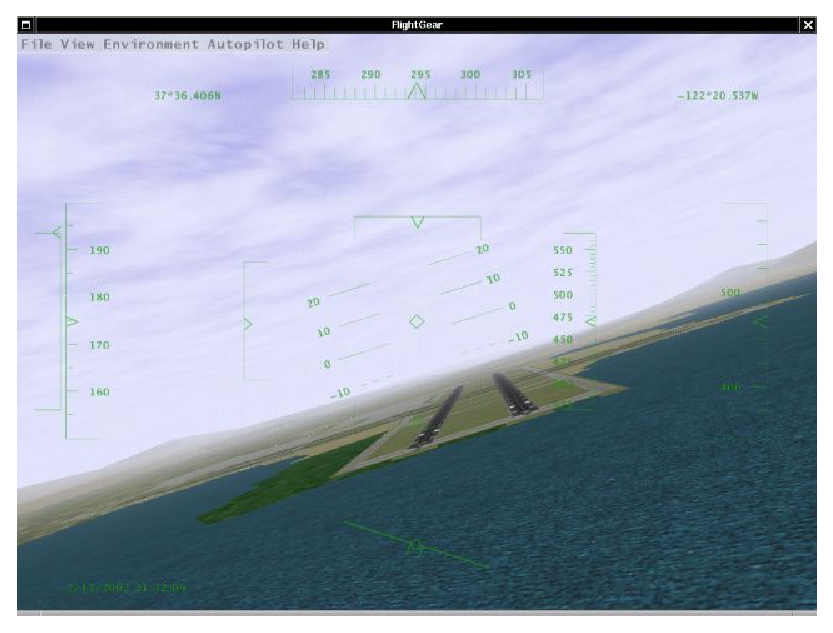
\includegraphics[clip,width=12.5cm]{KSFOapp}
}}

\smallskip
 \noindent
\iflanguage{english}{
Fig.\,1: \FlightGear{} under UNIX: \textit{Bad approach to San Francisco International - by one of the authors of this manual\ldots}
}{}
\iflanguage{french}{
Image 1 : \FlightGear{} sous UNIX: \textit{mauvaise approche de l'a\'{e}roport de San Francisco International, par l'un des auteurs de ce manuel\ldots}
}{}

%%%%%%%%%%%%%%%%%%%%%%%%%%%%%%%%%%%%%%%%%%%%%%%%%%%%%%%%%%%%%%%%%%%%%%%%%%%%%%%%%%%%%%%%%%%%%%%
\iflanguage{english}{
\section{System Requirements}\index{system requirements}
}{}
\iflanguage{english}{
\section{Pr\'{e}-requis syst\`{e}me}\index{system requirements}
}{}
%%%%%%%%%%%%%%%%%%%%%%%%%%%%%%%%%%%%%%%%%%%%%%%%%%%%%%%%%%%%%%%%%%%%%%%%%%%%%%%%%%%%%%%%%%%%%%%

\iflanguage{english}{
In comparison to other recent flight simulators, the \Index{system requirements} for
\FlightGear{} are not extravagant. A medium speed AMD Athlon64 or Intel
P4, even a decent AMD Athlon/K7 or an Intel PIII should be sufficient
to handle \FlightGear{} pretty well, given you have a proper 3D \Index{graphics
card}.

One important prerequisite for running \FlightGear{} is a graphics card whose driver supports
\Index{OpenGL}. If you don't know what \Index{OpenGL} is, the overview given at the OpenGL website
}{}
\iflanguage{french}{
En comparaison avec d'autres simulateurs de vol r\'{e}cents, les \Index{pr\'{e}-requis syst\`{e}me}
de \FlightGear{} ne sont pas exag\'{e}r\'{e}s. Un processeur AMD Athlon64 de vitesse moyenne, ou un
Intel P4, ou m\^{e}me un AMD Athlon/K7 d\'{e}cent ou un Intel PIII devraient \^{e}tre suffisants pour
faire fonctionner \FlightGear{} assez bien, pour peu que vous ayez une \Index{carte graphique} 3D appropri\'{e}e.

Un des pr\'{e}-requis les plus importants pour faire fonctionner \FlightGear{} est une carte graphique dont le
pilote prenne en charge \Index{OpenGL}. Si vous ne savez pas ce qu'est \Index{OpenGL}, la vue d'ensemble propos\'{e}e
sur le site Internet d'OpenGL : 
}{}
\medskip

\web{http://www.opengl.org}
\medskip

\noindent
\iflanguage{english}{
says it best: ``Since its introduction in 1992, OpenGL has become the
industry's most widely used and supported 2-D and 3D graphics application programming
interface (API)...''.

\FlightGear{} does not run (and will never run) on a graphics board which only supports
\Index{Direct3D}/\Index{DirectX}. Contrary to OpenGL, Direct3D is a proprietary interface, being restricted to
the Windows operating system.

You may be able to run \FlightGear{} on a computer that features a 3D video card not
supporting hardware accelerated \Index{OpenGL} -- and even on systems without 3D
graphics hardware at all. However, the absence of hardware accelerated OpenGL support can bring
even the fastest machine to its knees. The typical signal for missing hardware acceleration
are \Index{frame rate}s below 1 frame per second.

Any modern 3D graphics featuring \Index{OpenGL} support will do. For
\Index{Windows} video card drivers that support OpenGL, visit the home page of your video
card manufacturer. You should note that sometimes OpenGL drivers\index{OpenGL!drivers}
are provided by the manufacturers of the graphics chip instead of by the makers of the
board. If you are going to buy a graphics card for running \FlightGear{}, an NVIDIA GeForce
card is recommended, as these tend to have better OpenGL support than AMD/ATI Radeon. 256MB
of dedicated graphics memory will be more than adequate - many people run \FlightGear{} happily
on less.

To install the executable and basic scenery, you will need around 500 MB of free \Index{disk
space}. In case you want/have to compile the program yourself you will need about another
500 MB for the source code and for temporary files created during compilation. This does not
include the development environment, which will vary in size depending on the operating system
and environment being used.  Windows users can expect to need approximately 300 MB of additional
disk space for the development environment.  Linux and other UNIX machines should have most of
the development tools already installed, so there is likely to be little additional space
needed on those platforms.

For the \Index{sound effects}, any capable \Index{sound card} should suffice.
Due to its flexible design, \FlightGear{} supports a wide range of \Index{joysticks} and
\Index{yokes} as well as \Index{rudder pedals} under \Index{Linux} and \Index{Windows}. 
\FlightGear{} can also provide interfaces to full-motion flight chairs.

\FlightGear{} is being developed primarily under \Index{Linux}, a free UNIX clone
(together with lots of GNU utilities) developed cooperatively over the Internet in much
the same spirit as \FlightGear{} itself. \FlightGear{} also runs and is partly developed
under several flavors of \Index{Windows}. Building \FlightGear{} is also possible on a Mac OS X
and several different UNIX/X11 workstations. Given you have a proper \Index{compiler} installed,
\FlightGear{} can be built under all of these platforms. The primary compiler for all platforms is
the free \Index{GNU C++} compiler (the \Index{Cygnus} \Index{Cygwin} compiler under Win32).

If you want to run \FlightGear under Mac OS X, you need to have Mac OS X 10.4 or higher. 
Minimum hardware requirement is either a Power PC G4 1.0GHz or an Intel Mac, but We suggest 
you have MacBook Pro, Intel iMac, Mac Pro, or Power Mac (Power PC G5) for comfortable flight.
}{}

\iflanguage{french}{
l'explique tr\`{e}s bien : ``Depuis son introduction en 1992, OpenGL est devenue l'interface de
programmation d'application (Application Programming Interface, API) 2D et 3D la plus employ\'{e}e et
la mieux prise en charge de l'industrie...''.

\FlightGear{} ne fonctionne pas (et ne fonctionnera jamais) sur une carte graphique ne prenant en charge que \Index{Direct3D}/\Index{DirectX}.
Contrairement \`{a} OpenGL, Direct3D est une interface propri\'{e}taire, \'{e}tant limit\'{e}e au syst\`{e}me d'exploitation
Windows.

Vous devriez pouvoir faire fonctionner \FlightGear{} sur un ordinateur dot\'{e} d'une carte graphique 3D ne
prenant pas en charge l'acc\'{e}l\'{e}ration mat\'{e}rielle \Index{OpenGL} (et m\^{e}me sur des syst\`{e}mes sans
mat\'{e}riel graphique 3D du tout). Cependant, l'absence de prise en charge mat\'{e}rielle de l'acc\'{e}l\'{e}ration
OpenGL peut mettre sur les genoux m\^{e}me la plus rapide des machines. Les sympt\^{o}mes typiques de l'absence
d'acc\'{e}l\'{e}ration mat\'{e}rielle sont des \Index{taux d'images} (frame rate) inf\'{e}rieurs \`{a} 1 image par seconde. 

Toute carte graphique 3D moderne prenant en charge \Index{OpenGL} fera l'affaire. Pour les pilotes de
carte graphique \Index{Windows} qui prennent en charge OpenGL, visitez la page d'accueil de votre fabricant de
carte vid\'{e}o. Notez que, parfois, les pilotes OpenGL\index{OpenGL!drivers} sont fournis par les fabricants
des processeurs graphiques et non par les fabricants des cartes. Si \^{e}tes sur le point d'acheter une carte
graphique pour faire fonctionner \FlightGear{}, une carte NVIDIA GeForce est recommand\'{e}e, car elles ont
tendance \`{a} b\'{e}n\'{e}ficier d'une meilleure prise en charge OpenGL que les cartes AMD/ATI Radeon. 256 Mo
de m\'{e}moire graphique d\'{e}di\'{e}e sera plus qu'appropri\'{e} - de nombreuses personnes font fonctionner
\FlightGear{} sans souci avec moins.

Pour installer les ex\'{e}cutables et les sc\`{e}nes par d\'{e}faut, vous aurez besoin d'environ 500 Mo
d'\Index{espace disque} libre. Au cas o\`{u} vous voudriez/deviez compiler le programme vous-m\^{e}me, vous
aurez besoin d'\`{a} peu pr\`{e}s 500 Mo suppl\'{e}mentaires pour le code source et pour les fichiers temporaires
cr\'{e}\'{e}s durant la compilation. Cel\`{a} ne comprend pas l'environnement de d\'{e}veloppement, qui variera
en taille en fonction du syst\`{e}me d'exploitation et de l'environnement utilis\'{e}s. Les utilisateurs de Windows
peuvent s'attendre \`{a} avoir besoin d'approximativement 300 Mo d'espace disque suppl\'{e}mentaire pour l'environnement
de d\'{e}veloppement. Les machines fonctionnant sous Linux ou autres UNIX devraient avoir la plupart des outils de
d\'{e}veloppement d\'{e}j\`{a} install\'{e}s, il est donc probable qu'il ne faille que peu d'espace disque suppl\'{e}mentaire
sur ces plate-formes.

En ce qui concerne les \Index{effets sonores}, n'importe quelle \Index{carte graphique} devrait suffir. En raison de sa
conception flexible, \FlightGear{} prend en charge une large un large \'{e}ventail de \Index{joysticks}, de
\Index{manches} et de \Index{palonniers} sous \Index{Linux} et \Index{Windows}.
\FlightGear{} peut \'{e}galement fournir des interfaces aux si\`{e}ges de vol \textit{full-motion}.

\FlightGear{} est d\'{e}velopp\'{e} principalement sous \Index{Linux}, un clone libre et gratuit d'UNIX
(ainsi qu'un bon nombre d'outils GNU) d\'{e}velopp\'{e} coop\'{e}rativement via Internet dans plus ou moins
le m\^{e}me esprit que \FlightGear{} lui-m\^{e}me. \FlightGear{} fonctionne \'{e}galement et est en partie d\'{e}velopp\'{e}
sous plusieurs versions de \Index{Windows}. Il est \'{e}galement possible de compiler \FlightGear{} sur Mac OS X
ainsi que sur diverses stations de travail UNIX/X11. D\`{e}s l'instant o\`{u} vous disposez d'un \Index{compilateur} appropri\'{e}
install\'{e}, \FlightGear{} peut-\^{e}tre compil\'{e} sous toutes ces plate-formes. Le principal compilateur sur toutes ces plateformes
est le compilateur libre \Index{GNU C++} (le compilateur \Index{Cygnus} \Index{Cygwin} sous Win32).

Si vous voulez lancer \FlightGear{} sous Mac OSX, vous aurez besoin de Mac OS X 10.4 ou sup\'{e}rieur. Les pr\'{e}-requis minimums
sont soit un Power PC G4 \`{a} 1,0 GHz ou un Mac Intel, mais nous vous sugg\'{e}rons un MacBook Pro,
Intel iMac, Mac Pro ou Power Mac (Power PC G5) pour un confort de vol optimal.
}{}

%%%%%%%%%%%%%%%%%%%%%%%%%%%%%%%%%%%%%%%%%%%%%%%%%%%%%%%%%%%%%%%%%%%%%%%%%%%%%%%%%%%%%%%%%%%%%%%
\iflanguage{english}{
\section{Choosing A Version}\index{FlightGear!versions}
}{}
\iflanguage{french}{
\section{Choisir une version}\index{FlightGear!versions}
}{}
%%%%%%%%%%%%%%%%%%%%%%%%%%%%%%%%%%%%%%%%%%%%%%%%%%%%%%%%%%%%%%%%%%%%%%%%%%%%%%%%%%%%%%%%%%%%%%%

\iflanguage{english}{
It is recommended that you run the latest official release, which are typically produced annually,
and which are used to create the the pre-compiled binaries. It is available from
}{}

\iflanguage{french}{
Nous vous recommandons d'utiliser la derni\`{e}re version officielle, g\'{e}n\'{e}ralement produite
annuellement et qui est utilis\'{e}e pour cr\'{e}er les binaires pr\'{e}-compil\'{e}. Elle est disponible
\`{a} l'adresse :
}{}

\medskip

\web{http://www.flightgear.org/Downloads/}
\medskip
\iflanguage{english}{
If you really want to get the very latest and greatest (and, at times,
buggiest) code, you can clone the sources at
}{}
\iflanguage{french}{
Si vous voulez vraiment obtenir la toute derni\`{e}re version du code (la plus \'{e}volu\'{e}e et, parfois, la plus
instable), vous pouvez cloner les sources \`{a} partir de l'adresse :
}{}
 \medskip

\web{http://www.gitorious.org/fg}.

\iflanguage{english}{
to get the recent code. A detailed description of how to set this up for \FlightGear{}
can be found at
}{}
\iflanguage{french}{
pour obtenir le code le plus r\'{e}cent. Une description d\'{e}taill\'{e}e de la pr\'{e}paration de code en vue de l'ex\'{e}cution de
\FlightGear{} peut \^{e}tre trouv\'{e}e \`{a} l'adresse :
}{}
 \medskip

\web{http://wiki.flightgear.org/GIT}.



%%%%%%%%%%%%%%%%%%%%%%%%%%%%%%%%%%%%%%%%%%%%%%%%%%%%%%%%%%%%%%%%%%%%%%%%%%%%%%%%%%%%%%%%%%%%%%%
\iflanguage{english}{
\section{Flight Dynamics Models\label{flightmodels}}\index{flight dynamics model}\index{flight model}
}{}
\iflanguage{french}{
\section{Mod\`{e}les de dynamique de vol (Flight Dynamics Models, FDM)\label{flightmodels}}\index{Mod\`{e}les de dynamique de vol}\index{flight model}
}{}
%%%%%%%%%%%%%%%%%%%%%%%%%%%%%%%%%%%%%%%%%%%%%%%%%%%%%%%%%%%%%%%%%%%%%%%%%%%%%%%%%%%%%%%%%%%%%%%
\iflanguage{english}{
Historically, \FlightGear{} was based on a flight model it inherited (together
with the Navion airplane) from LaRCsim. As this had several limitations (most importantly,
many characteristics were hard wired in contrast to using configuration files), there were
several attempts to develop or include alternative \Index{flightmodels}. As a result,
\FlightGear{} supports several different flight models, to be chosen from at runtime.
}{}
\iflanguage{french}{
Historiquement, \FlightGear{} \'{e}tait bas\'{e} sur un mod\`{e}le de vol qu'il a h\'{e}rit\'{e} de LaRCsim (ainsi que l'avion Navion). Comme cela imposait plusieurs limitations (la plus importante, beaucoup de caract\'{e}ristiques
\'{e}taient cod\'{e}es en dur au lieu de passer par des fichiers de configuration), quelques tentatives ont
\'{e}t\'{e} faites pour d\'{e}velopper ou inclure des mod\`{e}les de vol alternatifs. En cons\'{e}quence,
\FlightGear{} prend aujourd'hui en charge diff\'{e}rents mod\`{e}les de vol, qui doivent \^{e}tre choisis au lancement
de l'application.
}{}

\begin{itemize}
\iflanguage{english}{
\item Possibly the most important one is the JSB flight model developed by Jon Berndt. The JSB
flight model is part of a stand-alone project called \JSBSim: 
}{}
\iflanguage{french}{
\item Le plus important est probablement le mod\`{e}le de vol JSB d\'{e}velopp\'{e} par Jon Berndt. Le mod\`{e}le
de vol JSB fait partie d'un projet autonome appel\'{e} \JSBSim:
}{} 

\web{http://jsbsim.sourceforge.net/}.

\iflanguage{english}{
\item Andrew Ross created another flight model called \YASim{}\index{YASim} for
\textit{Yet Another Simulator}. \YASim{} takes a fundamentally different approach to many other FDMs by
being based on geometry information rather than aerodynamic coefficients. \YASim{} has a particularly
advanced helicopter FDM.
}{}
\iflanguage{french}{
\item Andrew Ross a cr\'{e}\'{e} un autre mod\`{e}le de vol appel\'{e} \YASim{}\index{YASim} pour
\textit{Yet Another Simulator} (encore un autre simulateur). \YASim{} prend une approche fondamentalement diff\'{e}rente
de nombreux autres FDM, car il se base sur l'information g\'{e}om\'{e}trique plut\^{o}t que sur les coefficients a\'{e}rodynamiques.
\YASim{} dispose d'un FDM particuli\`{e}rement avanc\'{e} pour les h\'{e}licopt\`{e}res.
}{}

\iflanguage{english}{
\item Christian Mayer developed a flight model of a hot air
balloon. Curt Olson subsequently integrated a special ``UFO'' slew mode, which
helps you to quickly fly from point A to point B.
}{}
\iflanguage{french}{
\item Christian Mayer a d\'{e}velopp\'{e} le mod\`{e}le de vol d'un ballon \`{a} air chaud. Curt Olson int\'{e}gra ensuite un mode
de d\'{e}placement sp\'{e}cial, appel\'{e} ``UFO'', qui vous aide \`{a} voler rapidement d'un point A \`{a} un point B.
}{}

\iflanguage{english}{
\item Finally, there is the \Index{UIUC flight model}, developed by a
team at the University of Illinois at Urbana-Champaign. This work was 
initially geared toward modeling aircraft in icing conditions\index{icing!modelling}, but now
encompasses ``nonlinear'' aerodynamics, which result in more realism
in extreme attitudes, such as stall and high angle of attack flight.  Two 
good examples that illustrate this capability are the \Index{Airwave Xtreme 150} 
\Index{hang glider} and the 1903 \Index{Wright Flyer}. More details of the UIUC
flight model can be found at
}{}
\iflanguage{french}{
\item Enfin, il existe le \Index{mod\`{e}le de vol UIUC}, d\'{e}velopp\'{e} par une \'{e}quipe de
l'Universit\'{e} d'Illinois \`{a} Urbana-Champaign. Ce travail \'{e}tait initialement
tourn\'{e} vers la mod\'{e}lisation d'un a\'{e}ronef rencontrant des conditions de givrage\index{icing!modelling},
mais il inclut maintenant l'a\'{e}rodynamique ``non-lin\'{e}aire'', qui a pour cons\'{e}quence d'am\'{e}liorer le
r\'{e}alisme dans des attitudes extr\`{e}mes, comme le d\'{e}crochage et les vols \`{a} angle d'attaque \'{e}lev\'{e}.
Deux bons exemples qui illustrent cette capacit\'{e} sont le \Index{deltaplane} \Index{Airwave Xtreme 150} et le \Index{Wright Flyer} de 1903. De plus amples d\'{e}tails du mod\`{e}le de vol UIUC peuvent \^{e}tre obtenus \`{a} l'adresse :
}{}

\web{http://www.ae.illinois.edu/m-selig/apasim/Aircraft-uiuc.html}
\end{itemize}
\iflanguage{english}{
It is even possible to drive FlightGear's scene display using an external
FDM\index{FDM!external} running on a different computer or via named
pipe\index{FDM!pipe} on the local machine -- although this might not be a
setup recommended to people just getting in touch with \FlightGear{}.
}{}
\iflanguage{french}{
Il est m\^{e}me possible de piloter l'affichage de la sc\`{e}ne de \FlightGear{}
en utilisant un FDM externe\index{FDM!external} fonctionnant sur un ordinateur diff\'{e}rent ou
par l'interm\'{e}diaire d'un canal nomm\'{e} sur la machine locale (bien que cela ne soit pas
recommand\'{e} aux utilisateurs d\'{e}couvrant \FlightGear{}). 
}{}

%%%%%%%%%%%%%%%%%%%%%%%%%%%%%%%%%%%%%%%%%%%%%%%%%%%%%%%%%%%%%%%%%%%%%%%%%%%%%%%%%%%%%%%%%%%%%%%
\iflanguage{english}{
\section{About This Guide}
}{}
\iflanguage{french}{
\section{A propos de ce guide}
}{}
%%%%%%%%%%%%%%%%%%%%%%%%%%%%%%%%%%%%%%%%%%%%%%%%%%%%%%%%%%%%%%%%%%%%%%%%%%%%%%%%%%%%%%%%%%%%%%%

\iflanguage{english}{
\markright{\thesection.\hspace*{1mm} ABOUT THIS GUIDE}

There is little, if any, material in this Guide that is presented here exclusively. You
could even say with Montaigne that we ``merely gathered here a big bunch of other men's
flowers, having furnished nothing of my own but the strip to hold them together''. Most
(but fortunately not all) of the information herein can also be obtained from the
\FlightGear{} web site\index{FlightGear Website} located at
}{}

\iflanguage{french}{
\markright{\thesection.\hspace*{1mm} A PROPOS DE CE GUIDE}

Il y a peu, voire pas, de ressources dans ce guide qui y soient exclusivement présent\'{e}es.
Vous pourriez m\^{e}me dire comme Montaigne ``Je n'ai fait qu'un bouquet de fleurs et n'ai rien fourni
de moi-m\^{e}me que le lien qui les assemble.'' La majeure partie (mais heureusement pas
l'int\'{e}gralit\'{e}) des informations pr\'{e}sentes ici peut \'{e}galement \^{e}tre obtenue
\`{a} partir du site Internet de \FlightGear{} situ\'{e} \`{a} l'adresse : 
}{}

\medskip

\web{http://www.flightgear.org/}
\medskip

\iflanguage{english}{
\textit{The \FlightGear{} Manual} is intended to be a first step
towards a complete \FlightGear{} documentation\index{FlightGear
documentation}. The target audience is the end-user who is not
interested in the internal workings of \Index{OpenGL} or in building
his or her own scenery. It is our hope that someday there will be an
accompanying \textit{\FlightGear{} Programmer's Guide}\index{FlightGear
Programmer's Guide} 
a \textit{\FlightGear{} Scenery Design Guide},\index{FlightGear Scenery Design Guide}
describing the Scenery tools now packaged as \TerraGear{}; and a \textit{\FlightGear{}
Flight School}\index{FlightGear Flight School} package.
 \medskip

\textbf{We kindly ask you to help us refine this document by submitting corrections,
improvements, suggestions and translations. All users are invited to contribute
descriptions of alternative setups (graphics cards, operating systems
etc.). We will be more than happy to include those in future versions
of \textit{The FlightGear Manual} (of course not without giving credit
to the authors).}
}{}

\iflanguage{french}{
\textit{Le manuel \FlightGear{}} a pour vocation d'\^{e}tre un premier pas vers une
documentation compl\`{e}te de \FlightGear{}\index{FlightGear documentation}. Il s'adresse
\`{a} l'utilisateur final qui n'est pas int\'{e}ress\'{e} par le fonctionnement interne
d'\Index{OpenGL} ou par la cr\'{e}ation de ses propres sc\`{e}nes. Nous esp\'{e}rons qu'un
jour il y aura, pour accompagner ce document, un \textit{Guide du programmeur de \FlightGear{}}\index{FlightGear
Programmer's Guide}, un \textit{Guide de cr\'{e}ation des sc\`{e}nes de \FlightGear{}},\index{FlightGear Scenery Design Guide}
d\'{e}crivant les outils de sc\`{e}nes actuellement livr\'{e}s avec \TerraGear{}; et un paquetage \textit{Ecole de pilotage \FlightGear{}}\index{Ecole de pilotage FlightGear}.
 \medskip

\textbf{Merci de nous aider \`{a} am\'{e}liorer ce document en nous soumettant vos corrections, am\'{e}liorations, suggestions et traductions.
Tous les utilisateurs sont invit\'{e}s \`{a} contribuer aux descriptions des configurations alternatives (cartes graphiques, syst\`{e}mes d'exploitation, etc.). Nous serons plus qu'heureux de les inclure dans les futures versions du \textit{manuel FlightGear} (bien entendu sans oublier le cr\'{e}dit attribuable \`{a} leurs auteurs).}
}{}

%% Revision 0.00  1998/09/08  michael
%% Initial revision for version 0.53.
%% Revision 0.01  1998/09/20  michael
%% several extensions and corrections
%% revision 0.10  1998/10/01  michael
%% final proofreading for release
%% revision 0.11  1998/11/01  michael
%% minor corrections on platforms, satellite data, OpenGL
%% added Navion pic
%% revision 0.12  1999/03/07  michael
%% update on recent development
%% revision 0.20  1999/06/04  michael
%% updates on recent development, corrections of links
%% revision 0.3 2000/04/20 michael
%% Rewritten for version 0.7.2, many changes, added development since summer 1999,
%% development vs. stable version, split into SimGear/FlightGear/TerraGear
%% Proofread by Jon Berndt
%% revision 0.4 2001/05/12 michael
%% update on development during the last year, corrections on requirements,
%% new sections on different versions and on flight models
%% revision 0.41 2001/07/01 martin & michael
%% comment on external FDM
%% hint to FAQ
%% extended remarks on property manager
%% revision 0.5 2002/01/01 michael
%% several minor updates, corrected links
%% Hint on YASim by Martin
%% Picture KSFOapp added by Martin
%% System requirements contributed from Darrell
%% revision 0.6 2002/02/23 cameron
%% Many, many corrections
%% Rewrote several parts
%% Changed section titles
%% revision 0.6 2002/09/07 michael
%% Added contribution by M Selig on UIUC models
%% 3 minor typo/grammar edits by Dave Perry 
%% (P.12 replaced double apostrophe, p.14 <<<to to  >>> to, <<<users is >>>users are
%% Revision 16/10/08: spelling, grammar, syntax and typo corrections.
